\documentclass{beamer}
\usepackage[utf8]{inputenc}
\usepackage{amsmath}
\usepackage{multirow}
\usepackage{graphicx}
\usepackage{xcolor}
\usepackage{algpseudocode}

\title{\LARGE{My Hubris on Display}}
\subtitle{Nitpicking the pedagogical case study of two Stanford statisticians}
\author{Jared Cummings}
\date{Fall 2021}

\begin{document}

\maketitle

%%%%%%%%%%%%%%%%%%%%%%%%%%%%%%%%%%%%%%%%%%%%%%%%%%%%%%%%%%%
% 1
\begin{frame}{Data}
\begin{itemize}
    \item \small{Genotype data of 197 individuals at $m=100$ \textit{well-space} single-nucleotide polymorphism (SNP)}
    \item 29 individuals with missing values $implies$ $n = 168$
    \item Genotype of individual $i$ at locus $m$, $G_{im}$, is three level factor
    \begin{itemize}
        \item \tiny{two wild type genes: \texttt{AA} $\rightarrow 0$}
        \item one wild type, one mutation: \texttt{Aa} $\rightarrow 1$
        \item two mutations: \texttt{aa} $\rightarrow 2$
    \end{itemize}
    \item self-reported ethnicity reported
\end{itemize}


\begin{table}[h]
\centering
\label{tab:data_example}
\resizebox{\textwidth}{!}{%
\begin{tabular}{ccccccccc}
\hline
Subject & $\text{SNP}_1$ & $\text{SNP}_2$ & $\text{SNP}_3$ & \dots & $\text{SNP}_{97}$ & $\text{SNP}_{98}$ & $\text{SNP}_{99}$ & $\text{SNP}_{100}$\\
\hline
NA10852 & 1 & 1 & 0 & \dots & 1 & 1 & 0 & 0 \\
NA12239 & 1 & 1 & 0 & \dots & 1 & 1 & 0 & 0 \\
NA19072 & 0 & 0 & 0 & \dots & 0 & 0 & 0 & 0 \\
NA19247 & 0 & 0 & 2 & \dots & 0 & 0 & 0 & 2 \\
NA20126 & 2 & 0 & 0 & \dots & 2 & 0 & 0 & 0 \\
NA18868 & 0 & 0 & 1 & \dots & 0 & 0 & 0 & 1 
\end{tabular}%
}
\caption{\tiny{A subset of genotype data on 197 individuals, each with measurements at 100 SNPs. Each individuals \texttt{ethnicity} is known to be one of \texttt{Japanese}, \texttt{African}, \texttt{African American}, and \texttt{European}.}}
\end{table}

\end{frame}

%%%%%%%%%%%%%%%%%%%%%%%%%%%%%%%%%%%%%%%%%%%%%%%%%%%%%%%%%%%
% 2
\begin{frame}{Motivating model}
\begin{itemize}
    \item Efron and Hastie (2016) propose the model
    \begin{eqnarray}
        Z_{im}^{(c)} &\sim& \text{Multi}(1, Q_i)\\
        X_{im}^{(c)} | Z_{im}^{(c)} = j &\sim& \text{Bi}(1, P_{jm}) \notag\\
        Q_i &\sim& \text{Dir}(1, 1, 1) \notag\\
        P_{jm} &\sim& \text{Dir}(1,1). \notag
    \end{eqnarray}
    where $i$ indexes individuals, $m$ indexes loci, $c$ indexes gene copies
    \item $X_{im}$ is derived from $G_{im}$ by
    \begin{itemize}
        \item $G_{im} = 0 \implies X_{im} = (0, 0)$
        \item $G_{im} = 2 \implies X_{im} = (1,1)$
        \item $G_{im} = 1 \implies X_{im} = (0, 1) \lor X_{im} = (1, 0)$
    \end{itemize}
    \item Performs soft clustering of individuals on $\mathcal{S}_3$ with $Q_i$ as coordinates
\end{itemize}
\end{frame}

%%%%%%%%%%%%%%%%%%%%%%%%%%%%%%%%%%%%%%%%%%%%%%%%%%%%%%%%%%%
% 3
\begin{frame}{Criticism}

Efron and Hastie's model assumes more information than the data $G_{im}$ provide. Three cases:
\begin{enumerate}
    \item $\text{Pr}(G_{im} = 0) = \text{Pr}(X_{im} = (0, 0))$
    \item $\text{Pr}(G_{im} = 2) = \text{Pr}(X_{im} = (1, 1))$
    \item \color{red}$\text{Pr}(G_{im} = 1) = \text{Pr}(X_{im} = (0, 1)) + \text{Pr}(X_{im} = (1, 0))$
\end{enumerate}
\end{frame}

%%%%%%%%%%%%%%%%%%%%%%%%%%%%%%%%%%%%%%%%%%%%%%%%%%%%%%%%%%%
% 4
\begin{frame}{Questions}

What are the consequences of the model proposed by Efron and Hastie on estimating population admixture of \texttt{African Americans}...
\begin{itemize}
    \item ...as it relates to data representation?
    \item ...as it relates to the concentration parameters on $Q_i$?
\end{itemize}

\end{frame}

%%%%%%%%%%%%%%%%%%%%%%%%%%%%%%%%%%%%%%%%%%%%%%%%%%%%%%%%%%%
% 5
\begin{frame}{Proposed models}

For effect of concentration parameter
\begin{eqnarray}
Y_{im} | Q_i &\sim& \text{Multi}(1, Q_i)\\
G_{im} | Y_{im} = j, R_{jm} &\sim& \text{Multi}(1, R_{jm}) \notag\\
Q_i | \lambda_1, \lambda_2, \lambda_3 &\sim& \text{Dir}(\lambda_1, \lambda_2, \lambda_3) \notag\\
\lambda_k &\sim& \text{Gam}(2, 2) \notag \\
R_{jm} &\sim& \text{Dir}(1, 1, 1). \notag
\end{eqnarray}

For effect of data representation, same as above, but
\begin{eqnarray}
Q_i | \lambda_1, \lambda_2, \lambda_3 &\sim& \text{Dir}(\lambda_1, \lambda_2, \lambda_3) \\
\lambda_k &=& 1 \notag
\end{eqnarray}

\end{frame}

%%%%%%%%%%%%%%%%%%%%%%%%%%%%%%%%%%%%%%%%%%%%%%%%%%%%%%%%%%%
% 6
\begin{frame}{Model fitting}
\begin{itemize}
    \item All three models benefit from conjugacy -- Gibbs sampling used
    \item Model (2) uses Metropolis algorithm (3 univariate Gaussian random walks) for the posterior of hyperparameters $\lambda_k$
    \item More than 10 parameters are being estimated

\begin{table}[]
\centering
\caption{\tiny{Number of estimated parameters and effective number of parameters for the three models. The majority are the latent $Z_{im}^{(c)}$ and $Y_{im}$. Interest lies in the 168 $Q_i$ (504 values total described fully by 336).}}
\label{tab:my-table}
\begin{tabular}{l|rr}
          & $p_\text{actual}$ & $p_\text{WAIC}$ \\
          \hline
Model (1) & 34,704        & 2513.1      \\
Model (2) & 18,207        & 871.9       \\
Model (3) & 18,204        & 2058.3     
\end{tabular}
\end{table}

    \item Ordering of variables everywhere $j$ indexes can be permuted between chains and model fits
\end{itemize}
\end{frame}

%%%%%%%%%%%%%%%%%%%%%%%%%%%%%%%%%%%%%%%%%%%%%%%%%%%%%%%%%%%
% 7
\begin{frame}{Convergence}

\begin{enumerate}
    \item Run models for 10k iterations
    \item compute Raftery-Lewis diagnostic
    \item rerun at recommended settings
    \item Assess convergence with Geweke diagnostic
\end{enumerate}
    
\begin{table}[h]
\centering
\caption{\tiny{Settings for single chain convergence recommended by the Raftery-Lewis diagnostic. All models were refit using the recommended settings. The discrepancy between "by hand" implementations and those from NIMBLE, which automatically selects an algorithm or set of algorithms to use in estimation \citep{beraha2021}. Though it is likely that NIMBLE is preferring Gibbs sampling here, it is difficult to confirm that to be true. More advanced applications of NIMBLE overcome this uncertainty by allowing the user to directly specify the algorithm(s) used.}}
\label{tab:raftery-lewis}
\resizebox{\textwidth}{!}{%
\begin{tabular}{l|crrr}
\hline
 Implementation & Model & Thinning & Warm-up samples & Post-warm-up draws \\
          \hline
"By hand" & (1)   & 92       & 490             & 344632             \\
          & (2)   & 18       & 40              & 67428              \\
          & (3)   & 27       & 84              & 101142              \\
          \hline
NIMBLE    & (1)   & 33       & 126             & 123618             \\
          & (2)   & 16       & 66              & 59936              \\
          & (3)   & 39       & 154             & 146094          
\end{tabular}%
}
\end{table}

\end{frame}

%%%%%%%%%%%%%%%%%%%%%%%%%%%%%%%%%%%%%%%%%%%%%%%%%%%%%%%%%%%
% 8
\begin{frame}{Convergence (cont.)}
\begin{itemize}
    \item Geweke diagnostics appear to conform well with standard normal asymptotic behavior at convergence
    \begin{figure}[h]
	\centering 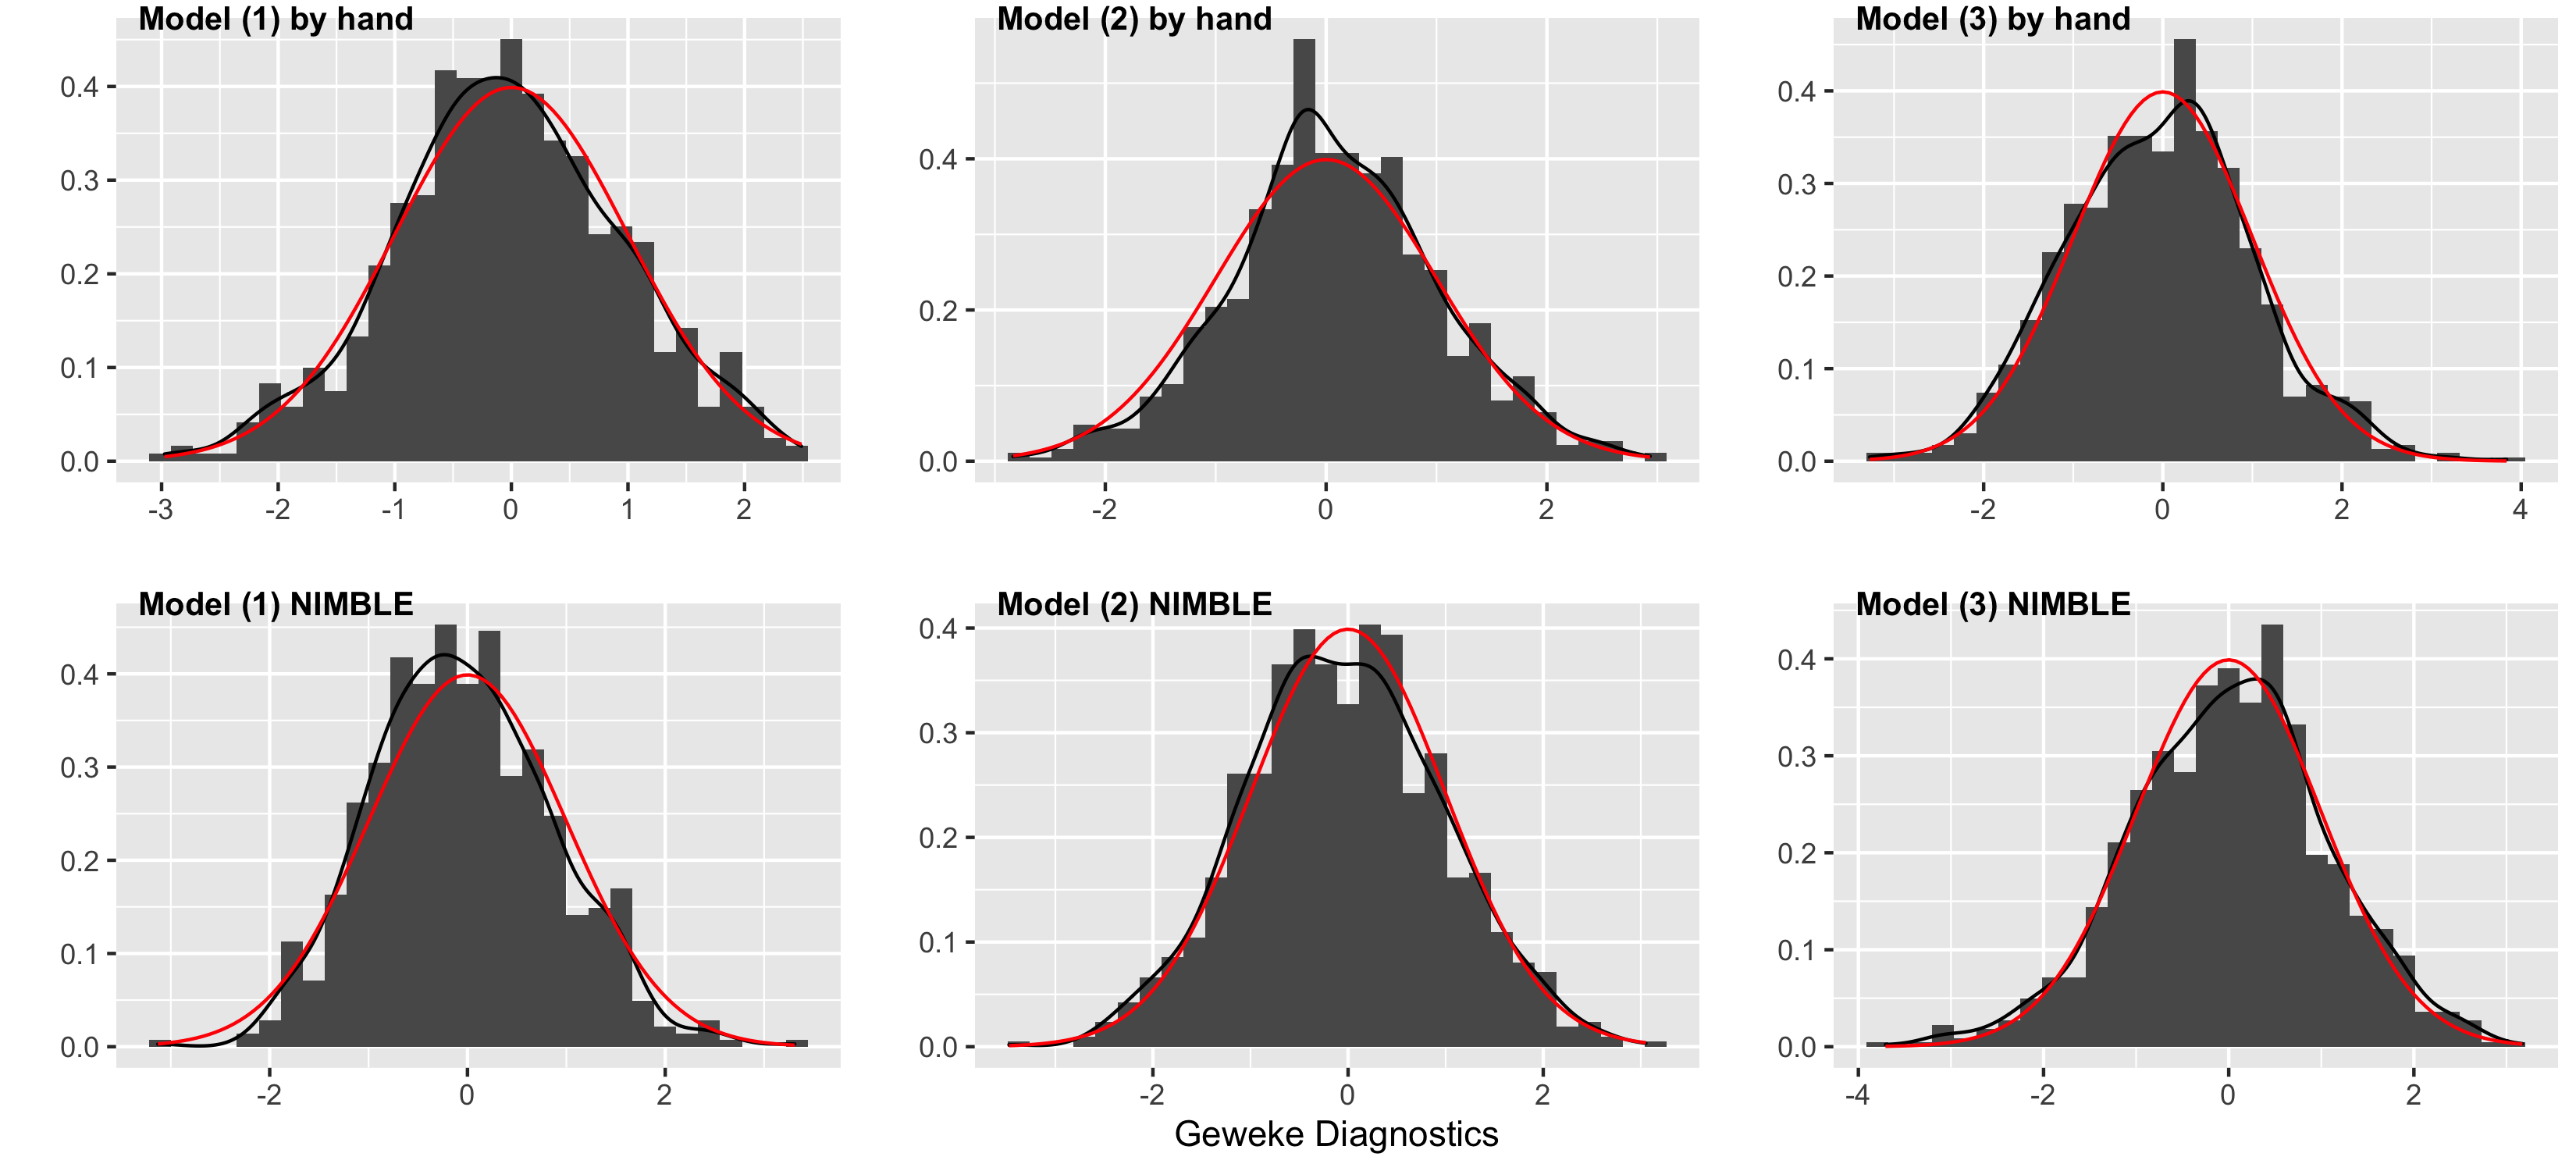
\includegraphics[width=0.8\textwidth]{SemesterProject/geweke_diags.png}
	\caption{\tiny{Geweke diagnostics for the six model fits given in histogram and KDE (black line) against a standard normal curve (red line). At convergence, Geweke diagnostics are asymptotically N(0,1). Slight bias exists in several of the displayed plots, but none of the plots appear heavy tailed.}}
	\label{fig:geweke}
\end{figure}
\end{itemize}


\end{frame}


%%%%%%%%%%%%%%%%%%%%%%%%%%%%%%%%%%%%%%%%%%%%%%%%%%%%%%%%%%%
% 9
\begin{frame}{Comparison of implementations}
\begin{itemize}
    \item \small{Problem: Parameter ordering and the number of parameters makes full comparison impractical}
    \item Solution: Let $T_i$ represent the ethnicity of individual $i$ as recorded in the data
\begin{equation*}
    \phi_t = \frac{1}{n_t} \sum_{i: T_i = t} \lVert T_i - \mu_t \rVert
\end{equation*}
    investigate conformity of $\phi_t$
    
    \begin{figure}[h]
	\centering 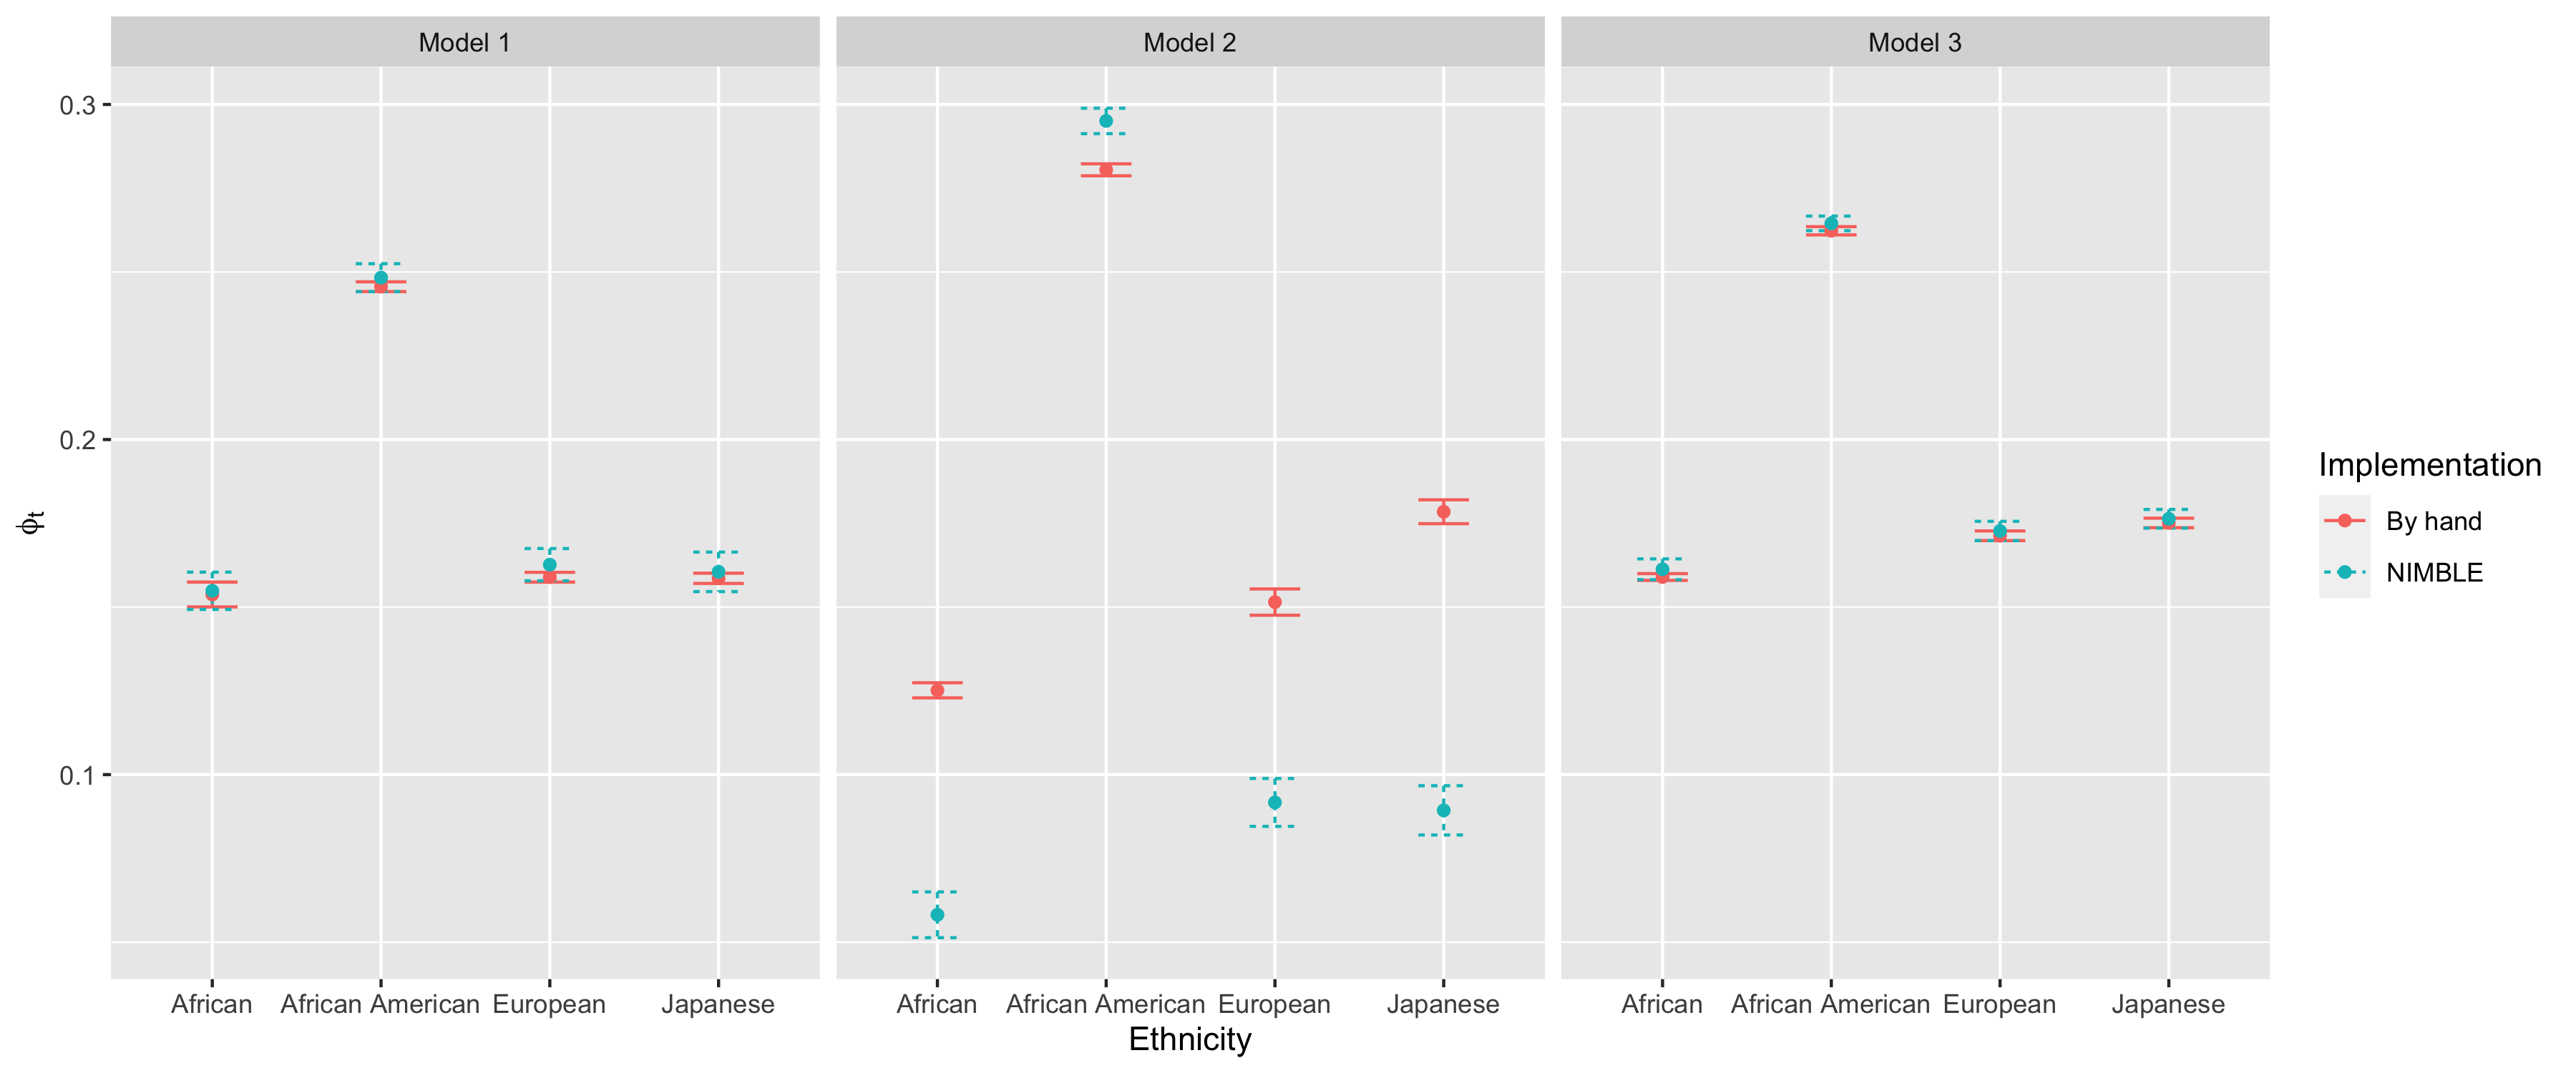
\includegraphics[width=0.8\textwidth]{SemesterProject/model_comp.png}
	\caption{\tiny{Comparison of implementations of the three models through the summary value $\phi_t$ with Monte Carlo error assessed. Both implementations fit similarly when estimating models 1 and 3. Model 2 displays non-trivial differences between implementations. It is interesting to note that between models 1 and 3, in all cases the point estimates of $\phi_t$ are lower for the model suggested by Efron and Hastie than for a model that does not reduce uncertainty by arbitrary data preprocessing. These estimates can be interpreted as strength of clustering, with lower values being associated with tighter clustering.}}
	\label{fig:model_comp}
\end{figure}
\end{itemize}
\end{frame}

%%%%%%%%%%%%%%%%%%%%%%%%%%%%%%%%%%%%%%%%%%%%%%%%%%%%%%%%%%%
% 10
\begin{frame}{Conformity of implementations (cont.)}

\begin{table}[]
\centering
\caption{\tiny{Estimates of concentration hyperparameters. Though inconclusive, the differences in estimates are likely due to differences in estimation procedures as they lead to similar expectations of the elements of $Q_i$ as shown in Table \ref{tab:expectations}.}}
\label{tab:concentration}
\resizebox{\textwidth}{!}{%
\begin{tabular}{ccrrrrr}
\hline
Implementation & Quantity  & Estimate & 95\% CrI LB & 95\% CrI UB  & 95\% MC LB & 95\% MC UB \\
\hline
By hand        & $\lambda_1$ & 0.261    & 0.190      & 0.346      & 0.260       & 0.261       \\
               & $\lambda_2$ & 0.374    & 0.284      & 0.471      & 0.373       & 0.374       \\
               & $\lambda_3$ & 0.508    & 0.418      & 0.611      & 0.507       & 0.508       \\
               \hline
NIMBLE         & $\lambda_1$ & 0.102    & 0.057      & 0.227      & 0.099       & 0.105       \\
               & $\lambda_2$ & 0.072    & 0.037      & 0.161      & 0.068       & 0.077       \\
               & $\lambda_3$ & 0.059    & 0.029      & 0.150      & 0.057       & 0.062      
\end{tabular}%
}
\end{table}

\begin{table}[]
\centering
\caption{\tiny{Estimates of the expected value of the elements of $Q_i$ a priori. Though the estimates of the two implementations are not equivalent up to Monte Carlo error, there are certainly strong similarities in reported values. Apparent differences have a likely source in the different estimated values of the concentration parameters reported in Table \ref{tab:concentration}. Note that the estimates in this table provide a good example of the ordering issue discussed previously.}}
\label{tab:expectations}
\resizebox{\textwidth}{!}{%
\begin{tabular}{ccrrrrr}
\hline
Implementation & Quantity    & Estimate & 95\% MC LB & 95\% MC UB  & 95\% CrI LB & 95\% CrI UB \\
\hline
By hand        & $Q_i{[}1{]}$ & 0.228    & 0.227      & 0.229      & 0.171       & 0.299       \\
               & $Q_i{[}2{]}$ & 0.327    & 0.327      & 0.327      & 0.258       & 0.394       \\
               & $Q_i{[}3{]}$ & 0.445    & 0.445      & 0.445      & 0.375       & 0.513       \\
               \hline
NIMBLE         & $Q_i{[}1{]}$ & 0.450    & 0.450      & 0.451      & 0.370       & 0.524       \\
               & $Q_i{[}2{]}$ & 0.306    & 0.306      & 0.306      & 0.242       & 0.374       \\
               & $Q_i{[}3{]}$ & 0.243    & 0.243      & 0.244      & 0.187       & 0.316      
\end{tabular}%
}
\end{table}
\end{frame}

%%%%%%%%%%%%%%%%%%%%%%%%%%%%%%%%%%%%%%%%%%%%%%%%%%%%%%%%%%%
% 11
\begin{frame}{Results and Sensitivity Analysis}
\begin{figure}
    \centering
    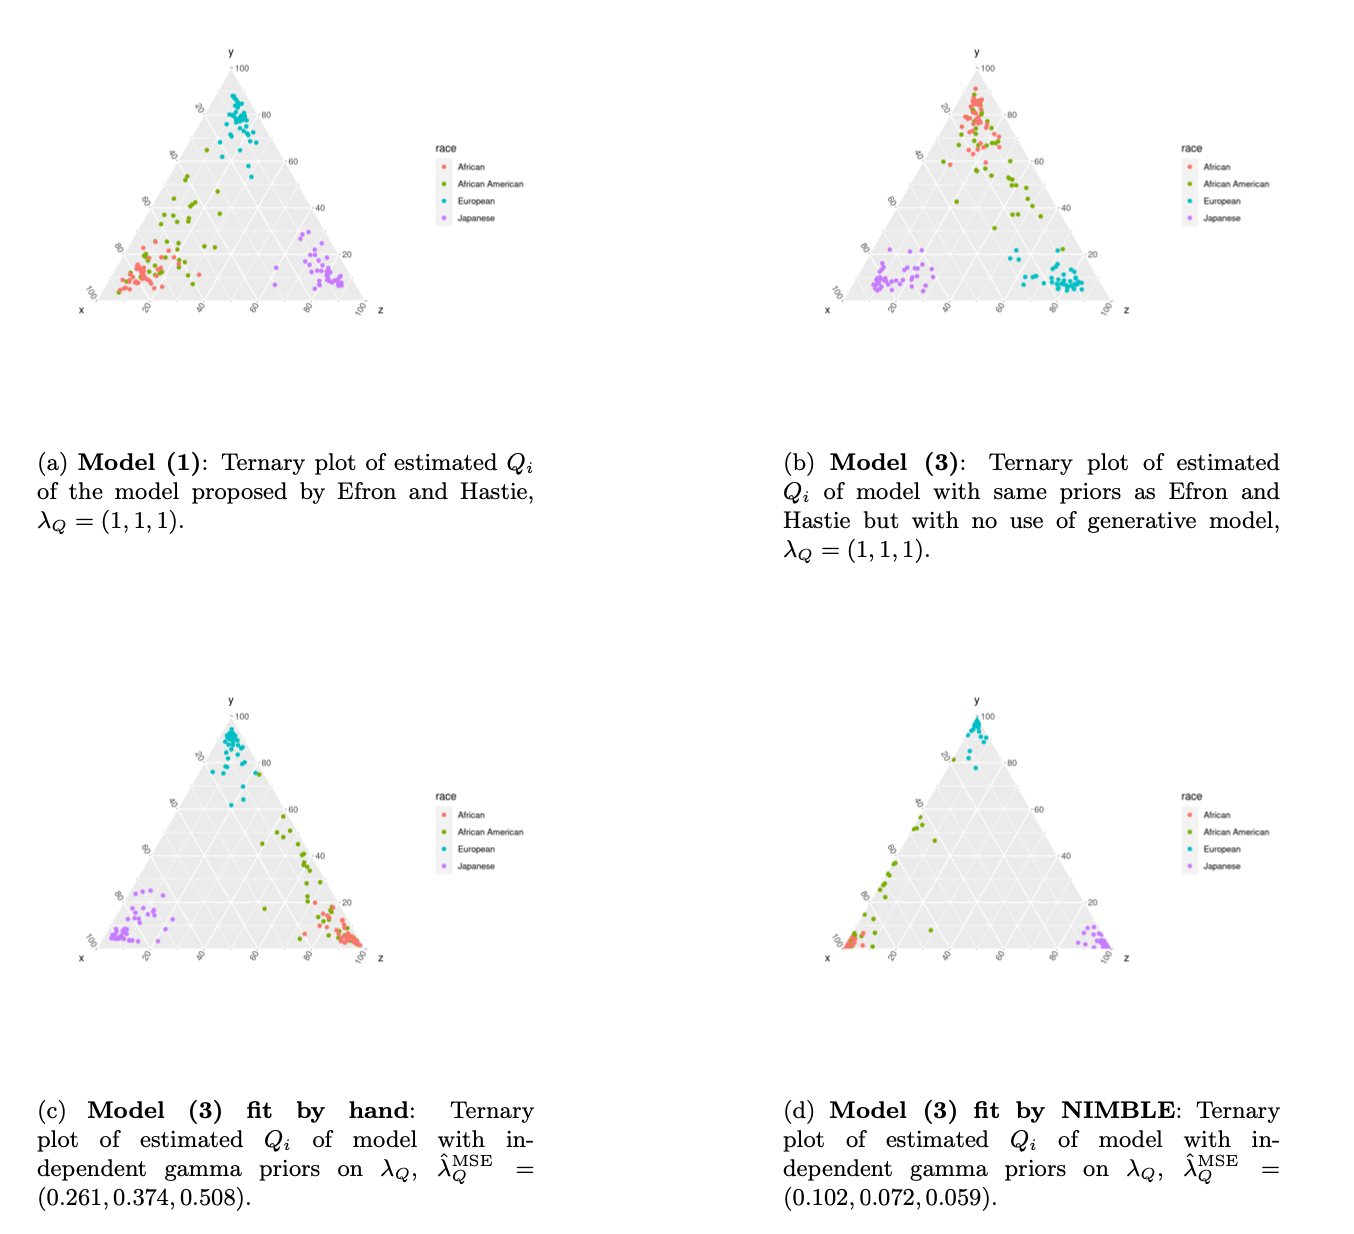
\includegraphics[width=0.8\textwidth]{SemesterProject/results_for_presentation.png}
    \label{fig:my_label}
\end{figure}
\end{frame}

%%%%%%%%%%%%%%%%%%%%%%%%%%%%%%%%%%%%%%%%%%%%%%%%%%%%%%%%%%%
% 12
\begin{frame}{Non-Bayesian Method}
\begin{itemize}
    \item Latent class models allow estimation of an analog to $Q_i$; EM algorithm + log-linear model
    \item Estimation issues when contingency table is sparse/cell counts are low
    \item (Highly subjective) variable selection can improve estimation and find meaningful clusters
    \begin{figure}
        \centering
        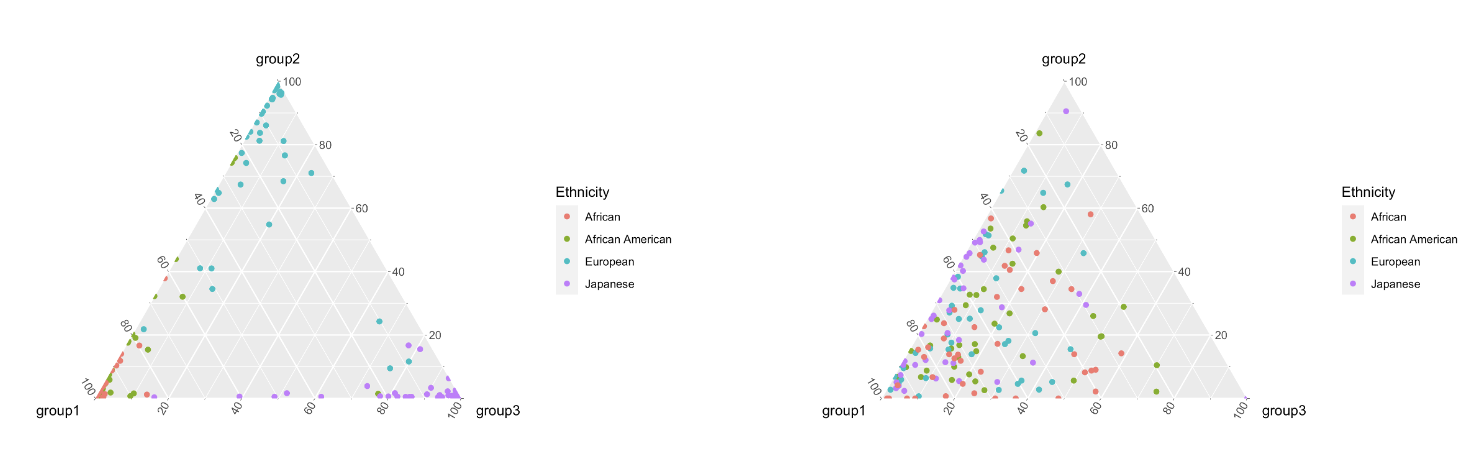
\includegraphics[width=0.8\textwidth]{SemesterProject/nonbayesian_method.png}
        \caption{\tiny{Estimation of admixture using a latent class model fit with 9 carefully selected SNP loci (left) and all SNP loci with empirical variance greater than 0 (right). Poor fit is to be expected with a sparse contingency table like the kind this data creates. Better clustering than this can be achieved with thoughtful variable selection, though this is a highly subjective process and the Bayesian method requires less input from the modeler.}}
        \label{fig:my_label}
    \end{figure}
    
\end{itemize}

\end{frame}

%%%%%%%%%%%%
\begin{frame}
\end{frame}


\bibliographystyle{plainnat}
\bibliography{project}
\end{document}
